\begin{minipage}[t][\PosterTopRowHeight][t]{\PosterTwoWidth}\vspace{0pt}
  \begin{TicketTwoPanel}{\PosterTopRowHeight}{2}{WHAT WE FOUND: WHICH MODE YOU PROTECT DECIDES}

    \noindent\begin{minipage}[c]{268mm}\centering
      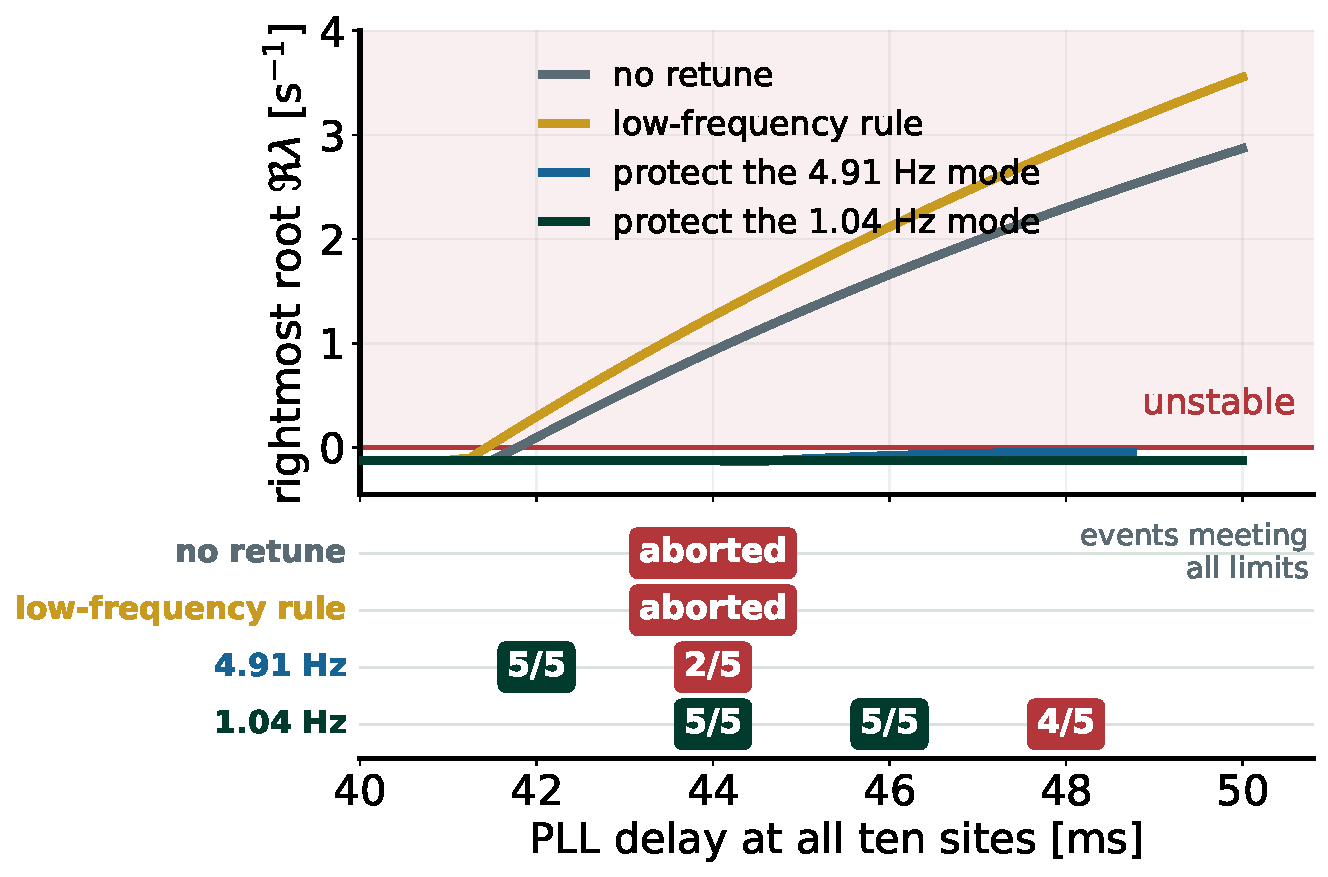
\includegraphics[width=266mm,height=175mm,keepaspectratio]{generated/figures/central.pdf}
    \end{minipage}\hfill%
    \begin{minipage}[c]{138mm}\raggedright
      {\FigureSize\textbf{At 44 ms (was 40 ms)}\par}\vspace{1mm}
      {\fontsize{22.5pt}{29pt}\selectfont
      \begin{tabular}{@{}l@{\ \ }c@{\ \ }c@{}}
        \textbf{rule} & \textbf{roots} & \textbf{events}\\\hline
        no retune & 8 / 10 & aborted\\
        low-frequency & 12 / 12 & aborted\\
        protect 4.91 Hz & 0 / 0 & 2 of 5\\
        protect 1.04 Hz & 0 / 0 & 5 of 5\\
      \end{tabular}\par}
      \vspace{2mm}
      {\fontsize{20pt}{23pt}\selectfont roots: unstable / beyond the $-0.05\ \mathrm{s^{-1}}$ margin, full-spectrum count. Events: five nonlinear load steps with frequency, RoCoF, voltage and SG-reserve limits.\par}
    \end{minipage}\par
    \vspace{1mm}
    \begin{InWords}\InWordsLabel The usual low-frequency compensation is worse than no retune. Protecting the least-damped 4.91 Hz mode restores the spectrum but uses up the frequency-response reserve. Protecting a well-damped 1.04 Hz mode keeps both.\end{InWords}

  \end{TicketTwoPanel}
\end{minipage}%
